%Especificacion
\documentclass[12pt]{article}

%Paquetes
\usepackage[left=2cm,right=2cm,top=3cm,bottom=3cm,letterpaper]{geometry}
\usepackage{lmodern}
\usepackage[T1]{fontenc}
\usepackage[utf8]{inputenc}
\usepackage[spanish,activeacute]{babel}
\usepackage{mathtools}
\usepackage{amssymb}
\usepackage{enumerate}
\usepackage{enumitem}
\usepackage{float}
%\usepackage{wasysym}
\usepackage{graphicx}
\graphicspath { {media/} }
%\usepackage{pifont}
\usepackage{titlesec}
\usepackage{amsmath}
\usepackage{hyperref}
\usepackage{multicol}
%Preambulo
\title{Seminario\\ Heurísticas de optimización combinatoria \\2017-2}
\author{Carlos Gerardo Acosta Hernández}
\date{Facultad de Ciencias UNAM \\ 3/04/17}
%\setlength\parindent{0pt}

\begin{document}
\maketitle
Como primer proyecto para el seminario de Heurísticas de optimización combinatoria,
se implementó un sistema para resolver instancias del \textbf{Problema del Agente Viajero} \footnote{Del inglés \textit{Traveling Salesman Problem (TSP)}}
en su versión simétrica, con la variación de ser un camino Hamiltoniano sin ciclo, como se describe usualmente.
Para lograr dicho cometido, utilizamos la heurística de \textbf{Recocido Simulado} \footnote{Del inglés \textit{Simulated Annealing}}.


\section{Sistema}
El sistema consta de los siguientes componentes:
\begin{itemize}
\item \textbf{Lenguaje de programación:} Scala 2.12.1
\item \textbf{Sistema de construcción:} SBT (\textit{Scala Build Tool}) 0.13.13
\item \textbf{Documentación:} ScalaDoc 2.12.1
\item \textbf{Graficación:} Gnuplot 5.0
\item \textbf{Insumos:} Los insumos (datos de entrada) fueron proporcionados por el profesor mediante una base de datos relacional \textit{SQL}. El sistema manejador de la base de datos utilizado es SQLite 3.16.2. El controlador del \textit{SMBD} es una biblioteca para \textit{Java} compatible con \textit{Scala}, SQLite-JDBC 3.16.1.
\item \textbf{Control de versiones:} Para mantener el control de versiones se utilizó Git 2.11.0 y el repositorio en línea se encuentra alojado en GitHub.
\end{itemize}
\subsection{Estructura}\label{sec:e}
El proyecto está organizado con la jerarquía de directorios que se
especifica para proyectos de \textit{SBT} (el sistema de construcción).
El árbol desde el directorio raíz, debe verse como:
\begin{verbatim}
    RecocidoSimulado-TSP/
    |__ doc/
    |__ lib/
    |__ src/
    |__ project/
    |__ src/
    |__ README.md
    |__ build.sbt
    |__ hi.db
    |__ conf.txt
\end{verbatim}

En la carpeta \textbf{doc}, se encuentra este documento que estás
leyendo, y su código fuente en \LaTeX; también un subdirectorio llamado
\textbf{graficas/} donde se almacena la gráfica de la última ejecución, reproducible con el archivo de captura \textit{graficas/gnuplot/}\textbf{exec.txt}. Para volver a generarla es necesario ejecutar el programa \textit{gnuplot} con \textit{graficas/gnuplot/}\textbf{commands.gp} de entrada.\\

En la carpeta de \textbf{lib}, se incluyen las bibliotecas externas al sistma de
construcción y al lenguaje de programación de las que depende el
proyecto. Sólo debe encontrarse por el
momento el driver del \textit{SMBD SQLite} para \textit{Java}. \\

Todo el código fuente referido a la implementación de la heurística
se encuentr en el directorio \textbf{src/}. Desde ahí es posible exploar
el código. Es importante recalcar que se incluye una carpeta para código
escrito en \textit{Java}, sin embargo, se encontrará vacía, pues la
implementación está realizada por completo con la sintáxis de \textit{Scala}. Hay dos subdirectorios en dicha sección, pero lo retomaremos más
adelante en diseño (Sección \ref{sec:c}).

En \textbf{project} están definidas las dependencias del proyecto en un
archivo de nombre \textbf{Dependencies.scala}, donde se definen las características del sistema de construcción (puede señalarse, por ejemplo, una versión específica de \textit{SBT} que será descargada en cuanto se inicialice el proyecto por la versión actual que tenga el sistema). Asimismo pueden agregarse todas las dependencias que sean necesarias, por el momento sólo se define la de \textit{ScalaTest} para pruebas unitarias.\\

Los archivos libres en la raíz se refieren a:
\begin{itemize}
\item \textit{README.md} es el archivo escrito en \textit{markdown} para
  la descripción del proyecto para el repositorio en línea.
\item \textit{build.sbt}  es el archivo de configuración del sistema,
  provee un nombre al proyecto, define la versión del lenguaje a utilizar, un empaquetador y conecta las dependencias externas del proyecto.
\item \textit{hi.db} es el archivo de la base de datos que \textit{SQLite} genera a partir de los insumos. Decidí incluirla para señalar
  dónde se espera que esté ubicada la base de datos en la ejecución del
  programa. 
\item \textit{conf.txt} es un archivo de configuración para una ejecución de la heurística. Por defecto contiene la instancia de 78 ciudades presentada en clase y la configuración de semillas y parámetros necesarios
  para obtener la mejor solución encontrada en la experimentación con el
  sistema, puede cambiarse su contenido, siempre que se respete el formato (su sintáxis será especificada en la Sección \ref{sec:d}). De cualquier forma, es la entrada del programa, por lo que podemos utilizar cualquier otro con la misma sintáxis.
\end{itemize}

\subsection{Diseño}\label{sec:c}
Para diseñar la heurística del Recocido Simulado, consideré implementar
interfaces para hacer la implementación independiente del
problema \textit{NP-Duro} con el que se fuera a trabajar. Sin embargo,
el uso de \textit{traits} en \textit{Scala} no es exactamente como
las interfaces de \textit{Java}, por lo que puede apreciarse en el código una dependencia importante con el \textit{TSP}. De cualquier forma, es posible intercambiar varias implementaciones de los traits sin que el Recocido se vea afectado del todo en su lógica -la función de costo, la condición de terminación, entre otros.

Como se mencionaba en la sección anterior, la implementación está dividida en dos paquetes principales, subdirectorios del paquete raíz.
\begin{verbatim}
    src/main/scala/
    |__ hoc/
    |__ autsp/
\end{verbatim}

El paquete \textbf{hoc} contiene todos los \textit{traits} del proyecto
y el paquete \textbf{autsp}\footnote{autsp se refiere a: Aceptación por umbrales TSP} contiene todas las implementaciones de dichos traits.
A continuación una lista enumerada de la relación entre cada implementación y el \textit{trait} que extiende.

\begin{multicols}{2}
\begin{enumerate}
\item CondicionDeTerminacion.scala
\item FitFun.scala
\item GeneradorVerificador.scala
\item Lote.scala
\item RecocidoSimulado.scala
\item Solucion.scala
\item Temperatura.scala
\end{enumerate}

\begin{enumerate}
\item MaximoFallidos.scala
\item FuncionDeCosto.scala
\item GenVer.scala
\item Lote.scala
\item AceptacionPorUmbrales.scala
\item Camino.scala
\item Temperatura.scala
\end{enumerate}
\end{multicols}

Para información más detallada de la implementación, favor de revisar
\textit{target/scala-2.12/api/}\textbf{index.html} con la \textit{API} generada por \textit{ScalaDoc}.


\subsection*{Uso}\label{sec:d}
\subsubsection*{Descarga del proyecto}
El proyecto se encuetntra alojado en línea en \textit{GitHub}, para
descargarlo basta ejecutar \textit{Git} en cualquier directorio del
sistema de archivos.
\begin{verbatim}
    $ git clone https://github.com/Pernath/RecocidoSimulado-TSP.git
\end{verbatim}
Se creará un directorio con la estructura definida en la sección \ref{sec:d}.
\subsubsection*{Compilación y ejecución}
Para las operaciones siguientes se supone que el sistema operativo ya cuenta con el sistema de construcción \textit{sbt} instalado.\\

\noindent
En primer lugar llamamos al sistema de construcción, que buscará el
archivo \textbf{build.sbt} y establecerá la ruta actual como la ruta
del proyecto.
\begin{verbatim}
    [user@host RecocidoSimulado-TSP]$ sbt
\end{verbatim}
Esto nos llevará a un \textit{prompt} desde el que podremos llamar
los siguientes comandos de acuerdo a lo que necesitemos.

Para compilar el proyecto y verificar que todo está listo para las pruebas, ejecutamos
\begin{verbatim}
    > compile
\end{verbatim}
Posteriormente, será posible ejecutar el programa con el archivo de configuración como argumento.
\begin{verbatim}
    > run conf.txt
\end{verbatim}

Si deseamos guardar la ejecución para poder graficarla con \textit{gnuplot} o algún otro programa que acepte el formato ``<x>\; <y>'' en cada línea, ejecutamos con un segundo argumento `w'\footnote{Es muy importante señalar que si empaquetamos el proyecto y ejecutamos el \textit{JAR}, esta función dejará de estar disponible, pues la ruta establecida para escribir la ejecución
es dependiente de la estructura de directorios del sistema. No lo recomiendo y definitavemente pensaré en una alternativa, pero siempre se puede reproducir la ruta que realizará el programa para buscar el archivo \textbf{exec.txt}.}. 
\begin{verbatim}
    > run conf.txt w
\end{verbatim}
\subsubsection*{Empaquetado}
Una manera de empacar la implementación es ejecutar el siguiente comando:
\begin{verbatim}
    > package
\end{verbatim}
Sin embargo, este no incluirá las dependencias externas en el \textit{JAR} generado bajo la ruta \textit{target/scala-2.12/}\textbf{AUTSP.jar}, por lo que no será portátil y dependerá \underline{siempre} de la estructura de directorios del sistema.

Por fortuna, también incluí la opción para generar un \textit{stand-alone JAR} que nos permitirá mover líbremente el ejecutable de \textit{Java} y ejecutarlo desde cualquier directorio. Esto se logra con el
siguiente comando y podrá encontrarse el ejecutable en la misma dirección mencionada anteriormente:
\begin{verbatim}
    > assembly
\end{verbatim}

\subsubsection*{JAR y requisitos}
Cómo se había mencionado anteriormente, para poder ejecutar el sistema como producto de \textit{assembly}, es necesario que mantengamos tanto
la base de datos \textbf{hi.db} al mismo nivel de directorio y que conseve ese nombre, pues a diferencia de \textbf{conf.txt} no es un argumento
del programa y siempre se referirá a este en sus ejecuciones.
\begin{verbatim}
    [user@host scala-1.12]$ java -jar AUTSP.jar conf.txt
\end{verbatim}

\subsubsection*{Archivo de configuración}
El archivo de configuración por defecto que se incluye desde el repositorio en línea es \textbf{conf.txt}. Puede utilizarse cualquier otro archivo o modificar este para que el sistema produzca nuevos resultados, si
la entrada es la misma, el sistema reproducirá su ejecución. El archivo
debe contar con dos líneas únicamente, al menos sólo dos serán leídas.
\\


En la primera, separadas por comas y \underline{sin espacios}, deben ir las ciudades de la instancia de \textit{TSP}
con la que se trabajará:
\begin{verbatim}
                      [id_city_a],[id_city_b],...,[id_city_w]
\end{verbatim}
Donde $a,b,w \leq 278$.\\

La segunda y última línea, contiene los parámetros de la ejecución,
igualmente separados por comas \underline{sin espacios}:

\begin{verbatim}
[semilla],[temp_inicial],[phi],[tamaño_lote],[epsilon],[epsilonP],[constante_costo]
\end{verbatim}

\newpage
\section{Experimentación}
Para la experimentación, utilicé la instancia de \textit{TSP} que nos
proporcionó el profesor de 78 ciudades.
Aquí la lista de los id's de las ciudades incluídas en la instancia:\\

[1, 5, 9, 12, 16, 22, 23, 29, 30, 31, 39, 48, 52, 56, 58, 62, 65, 66, 70, 75, 80, 84, 86, 90, 92, 94, 95, 101, 107, 117, 119, 122, 133, 135, 143, 144, 146, 147, 150, 158, 159, 160, 166, 167, 176, 178, 179, 185, 186, 188, 190, 191, 194, 198, 200, 203, 207, 209, 213, 215, 216, 220, 221, 224, 227, 232, 233, 235, 238, 241, 244, 248, 250, 254, 264, 266, 274, 276]
\\


La experimentación se llevó a cabo en dos computadoras distintas:\\

\textbf{1.} Memoria RAM: 7.7GiB

Procesador: Intel Core i5 CPU @ 2.40GHz x 4\\

\textbf{2.} Memoria RAM: 3.9GiB

Procesador: AMD E-3 CPU @ 1.60GHz x 2\\

Se probaron alrededor de 1000 semillas distintas con resultados con de muy mala evaluación aunque factibles y 20 pruebas más, una vez encontrada la configuración de parámetros más favorable con evaluaciones a lo más de $0.5$.
\subsection*{Parámetros elegidos}
Los parámetros elegidos son los siguientes:
\begin{itemize}
\item Semilla: 14
\item Temperatura inicial: 4
\item \textbf{$\varphi$}: 0.9
\item Tamaño de lote: 10,000
\item \textbf{$\varepsilon$}: 0.001
\item \textbf{$\varepsilon_p$}: 0.04
\item \textbf{$C$}: 3
\end{itemize}
\newpage
\subsection*{Mejor solución encontrada}
A continuación se presenta una gráfica con de las soluciones aceptadas
y su evaluación para la mejor configuración de parámetros.
\begin{figure}[H]
  \centering
  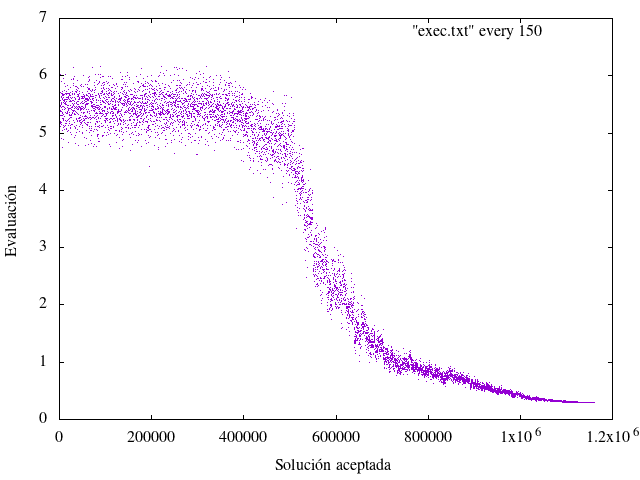
\includegraphics[width=1\textwidth]{mejor}
  \caption{Gráfica de la mejor configuración encontrada.}
\end{figure}

El producto final de dicha corrida es un camino factible con evaluación
de 0.28967526729032445:\\

[1, 188, 95, 144, 233, 9, 80, 250, 146, 147, 276, 274, 58, 224, 158, 31, 213, 22, 185, 29, 266, 133, 227, 254, 84, 66, 159, 216, 5, 143, 248, 23, 176, 122, 209, 62, 90, 203, 235, 52, 215, 70, 75, 198, 220, 92, 179, 16, 241, 190, 244, 186, 232, 238, 48, 12, 107, 264, 191, 221, 150, 86, 166, 135, 119, 94, 207, 56, 30, 65, 101, 200, 167, 160, 178, 194, 39, 117]

\section{Conclusiones}
Aunque tardé bastante más en la experimentación de lo que tenía contemplado -provocando que el refinamiento del sistema no fuera el deseado-
estoy bastante satisfecho con el resultado final obtenido. A decir verdad la experimentación que realicé en un principio no parecía ser suficiente por los resultados encontrados. Esto resultó ser bastante frustrante. No fue hasta que hice con detenimiento las pruebas, considerando los cambios que podía experimentar el sistema, que por fin di con una configuración apropiada y hubo oportunidad
de probar un número significativamente menor que en las primeras pruebas (de 1000 a sólo 20). Aún con la mejora visible en la evaluación de los
resultados (los exhibidos en la última clase eran de entre 0.7 a 1), y ahora contar con uno muy cercano a la mejor encontrada por el grupo, creo que es necesario continuar la experimentación de mi sistema y mejorar la interfaz del usuario. 

Como primer proyecto de clase, creo que fue muy importante llevarlo a
término para tener más herramientas y planificar con mayor eficiencia
el siguiente. La oportunidad de implementar una nueva heurística,
me proveerá de una más amplio panorama de elección para el nuevo proyecto. 
\end{document}